\documentclass[a4paper]{article}

%% Language and font encodings
\usepackage[english]{babel}
\usepackage[utf8x]{inputenc}
\usepackage[T1]{fontenc}

%% Sets page size and margins
\usepackage[a4paper,top=3cm,bottom=2cm,left=3cm,right=3cm,marginparwidth=1.75cm]{geometry}

%% Useful packages
\usepackage{amsmath}
\usepackage{graphicx}
\usepackage[colorinlistoftodos]{todonotes}
\usepackage[colorlinks=true, allcolors=blue]{hyperref}

\title{Assignment 3}
\author{Christa Wright (wrighch3),\\ Kuan-Yu Lai,\\ Blake Hudson(hudsonbl), \\Eric Sisson (sissone), \\ Jorge Guzman Nader(guzmannj)}

\begin{document}
\maketitle
\tableofcontents
\pagebreak
\section{User Interface Prototypes}
The main page displays a title, navigation bar containing five options; Login, Home, Goals, Nutrition and Contact Us. The middle of the page is reserved for the user to interact with the program. Besides the navigation bar. The bottom of the page will display regular web page signatures such as About Us, Search etc. The level bar on the bottom of the screen tracks the users experience gained from accomplishing goals. The web-page will follow the format described above for each web page.

\subsection{Home Page}
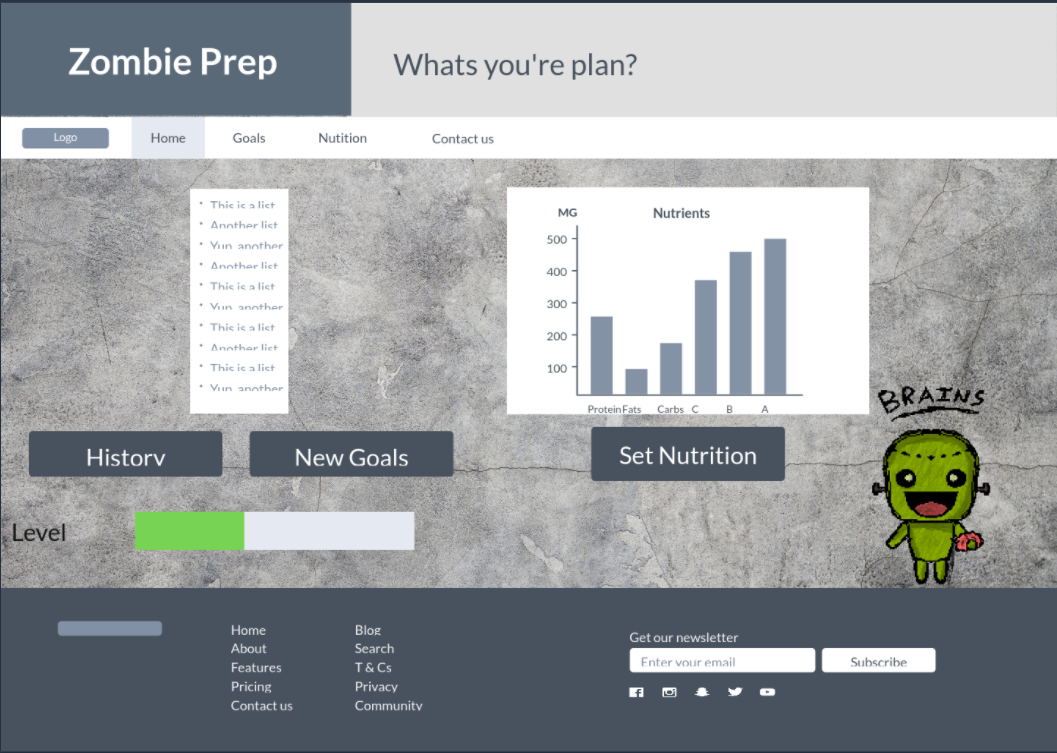
\includegraphics[width=\textwidth]{HomePage.PNG}

The main page displays three different selectable options; Goals, and Nutrition. The level bar on the bottom of the screen tracks the users experience gained from accomplishing goals. Based on the input from the nutritional goals page, the output gets printed to this page.

\subsection{Nutrition Goals}
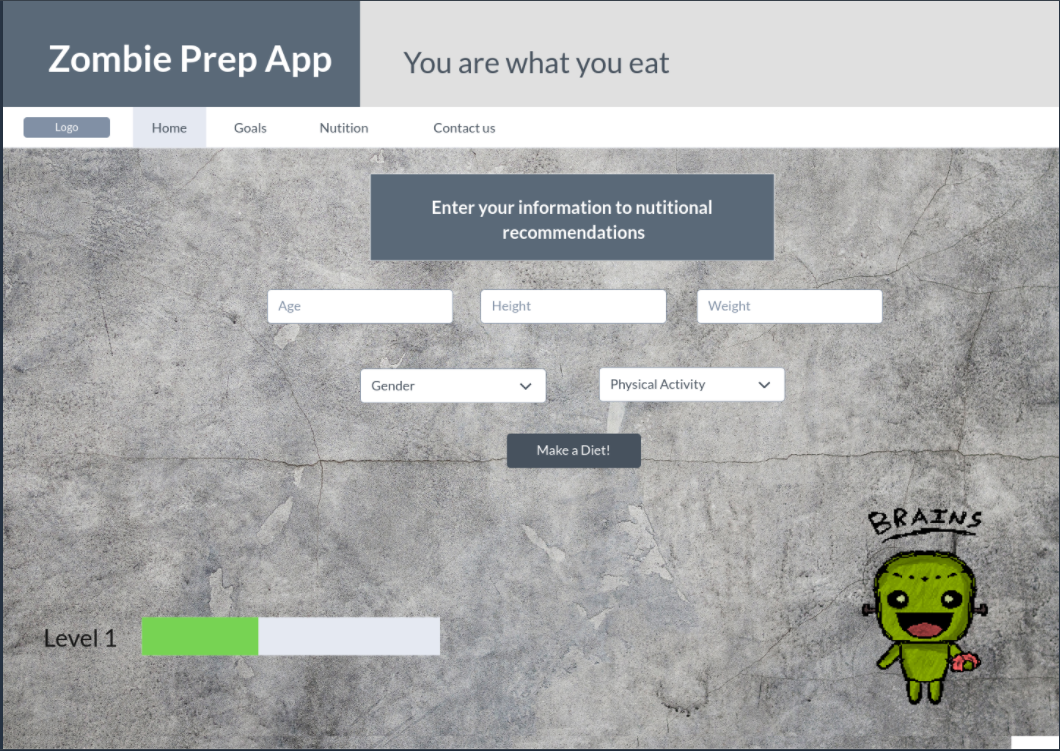
\includegraphics[width=\textwidth]{Nutrition.PNG}
If the user selects the Nutrition feature, the user will be redirected to this page. The user enters in data pertaining to their age, height, weight, and productivity. All of the data gets calculated using nutrition and metabolic equations that will output a detailed nutritional chart which contains quantities of nutriments( protein, carbs, lipids, vitamins, minerals) in a tabulated manner, that will be intuitive for the user to understand.

\subsection{Goals Page}
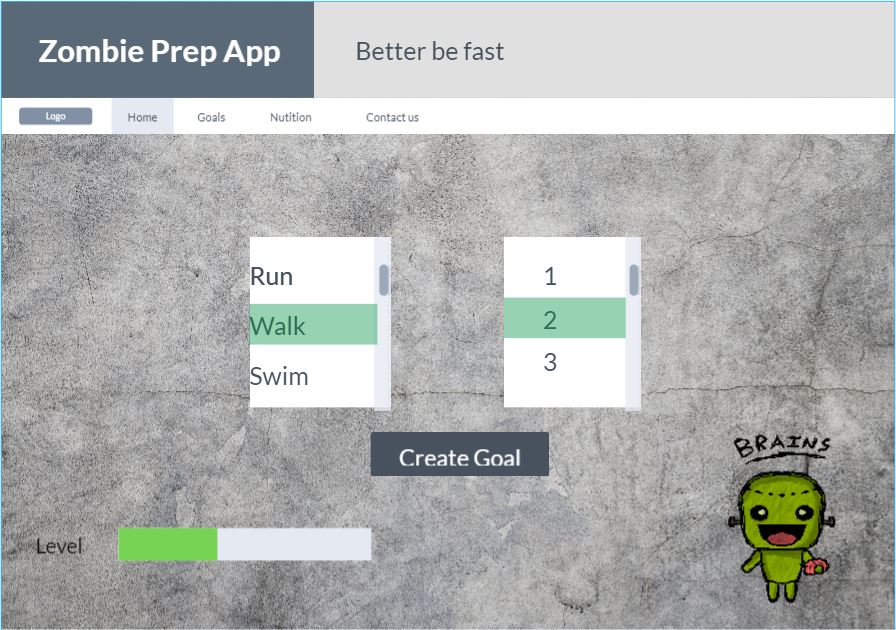
\includegraphics[width=\textwidth]{SetGoals.JPG}
In the goals page the user will be interfaced with three intractable templates. The first two are meant for generating user data. They have options of workouts, and data according to the input. Then lastly there is a button to create the goal.

\pagebreak
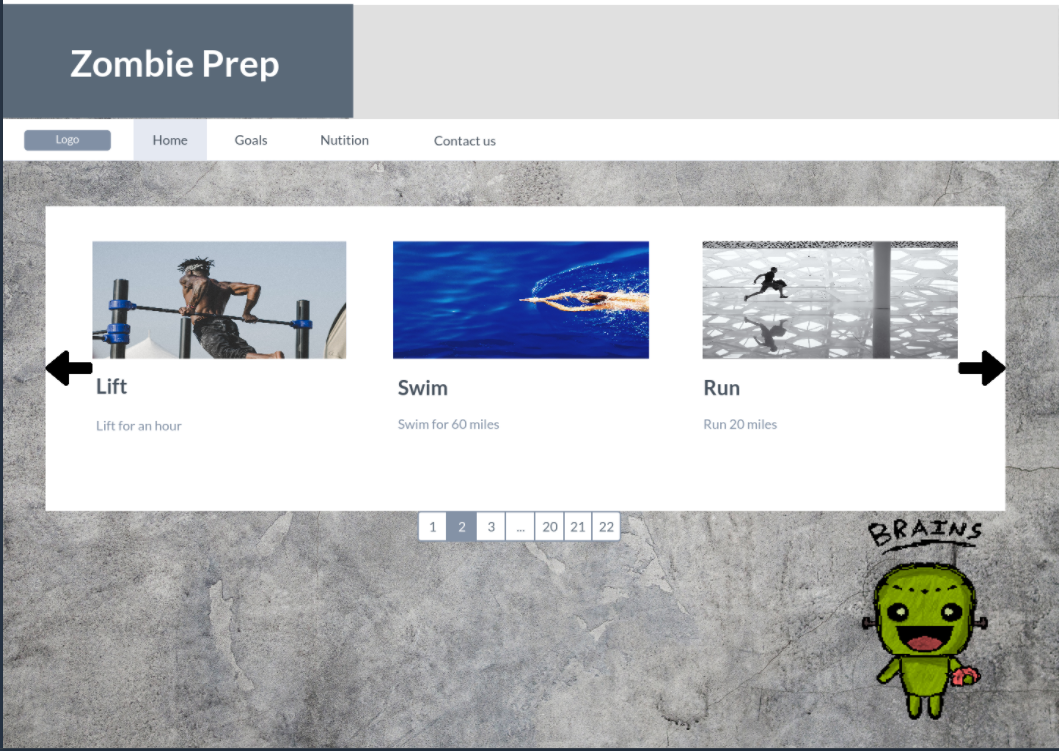
\includegraphics[width=\textwidth]{Goals2.PNG}
The image above displays all of the past goals the user generated from the use of the application. 
\pagebreak
\subsection{History}
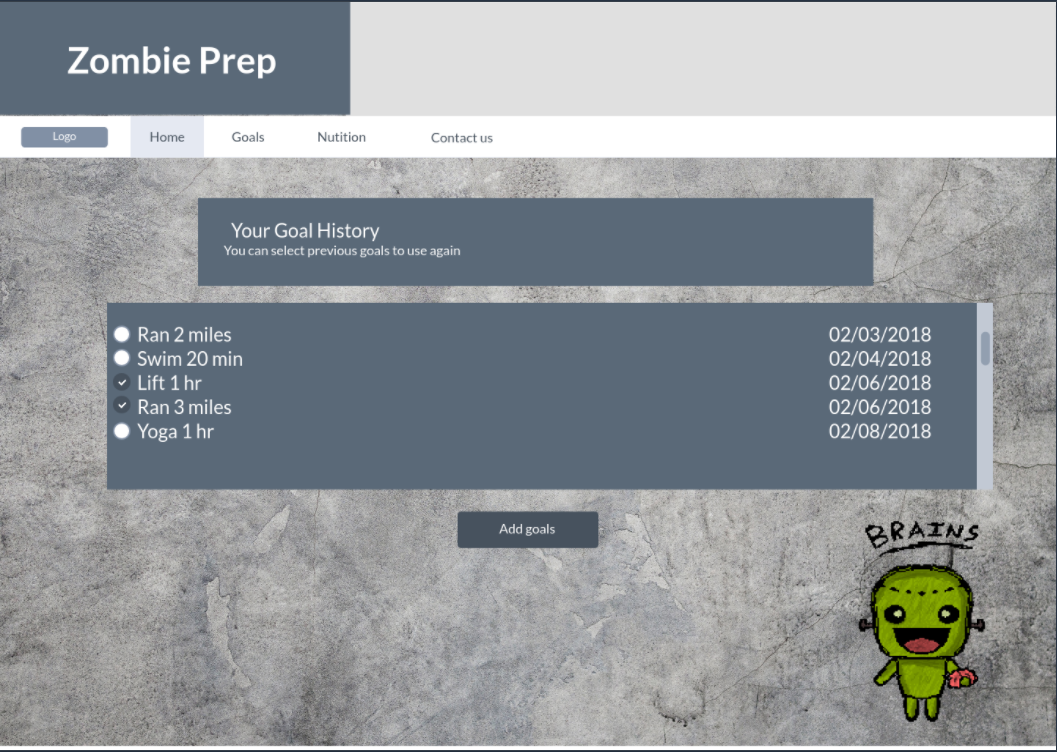
\includegraphics[width=\textwidth]{History.PNG}
The History page displays past goals that have been achieved. There isn't any user interactivity on this page.

\pagebreak
\subsection{Not Found Page}
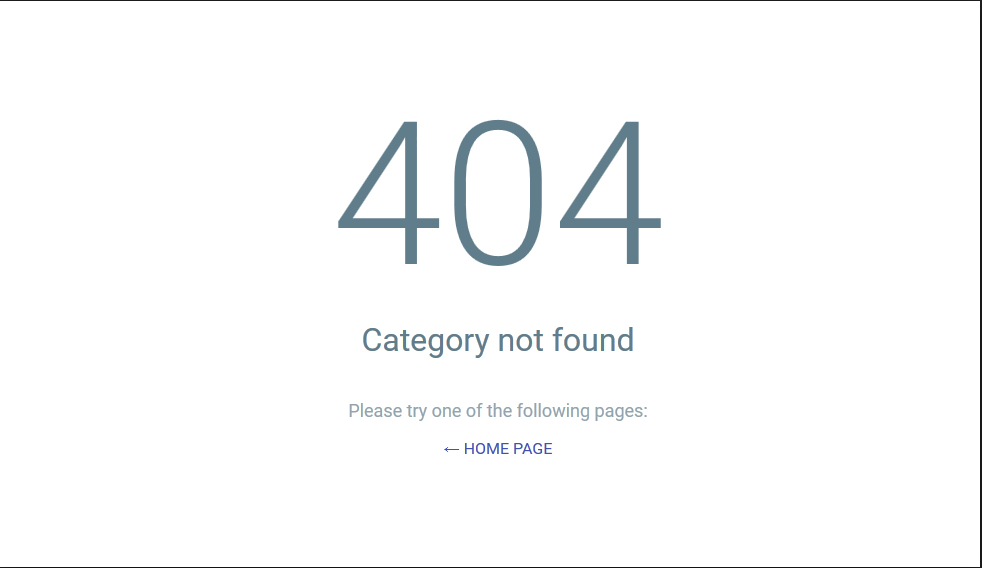
\includegraphics[width=\textwidth]{404Page.PNG}
This page will be selected if the user enters wrong url information.

\pagebreak
\section{Class Diagrams}
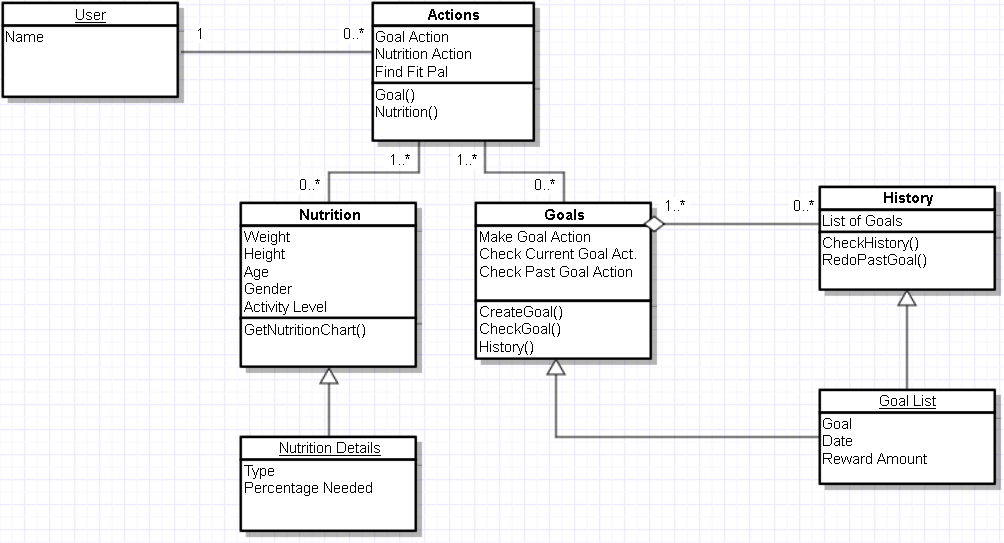
\includegraphics[width=\textwidth,height=11cm]{ClassDiagram.PNG}
The classes that will be focused on most are the Goals, Nutrition, and History classes.  The user will use these three classes based on the actions that they take.  The Goals class will be used to create goals, check the current goal, and access the History class.\\
The History class will keep track of past goals and allow the user to check their past, completed goals.  They will also be able to add one of their past goals to their current goal list.  The Nutrition Chart will take several variables from the user to create a nutrition chart.  The variables include weight, height, gender, age, and activity level.  The nutrition chart will show what how much the user should eat and what types of food they should eat.
\section{Sequence Diagrams}

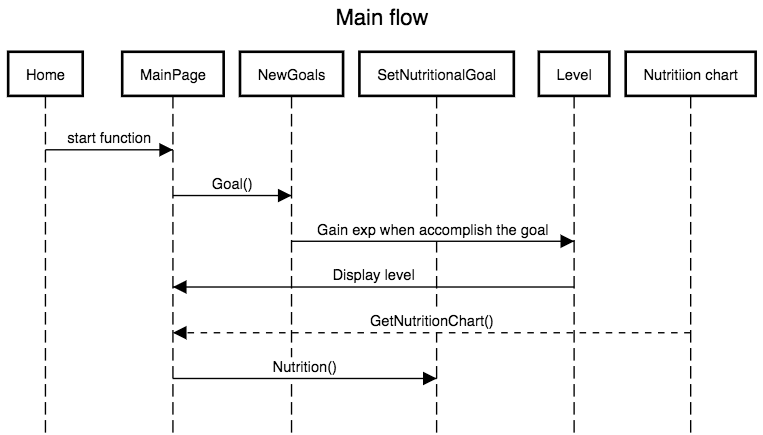
\includegraphics[width=\textwidth,height=10cm]{Main_flow.png}
\newline
\newline
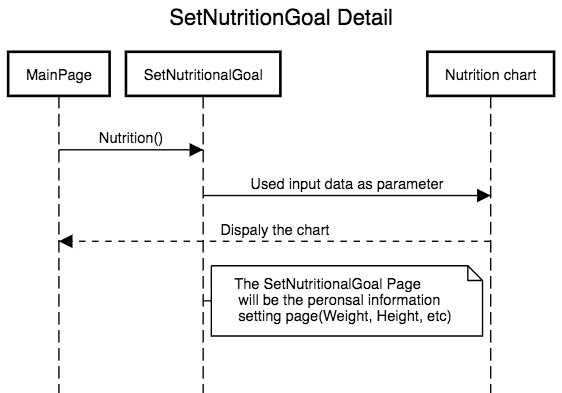
\includegraphics[width=\textwidth,height=10cm]{SetNutritionGoal_Detail.png}
\newline
\newline
\newline
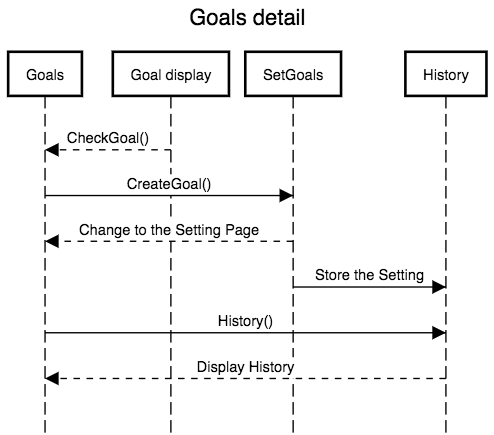
\includegraphics[width=\textwidth,height=10cm]{Goals_detail.png}
\newline
\section{Meeting Report}

\subsection{Progress made this week}

This week we decided to used web languages such as css, html, nodejs, javascript because of their portability and ease to implementation. We focused our attention in how the user interface for the application will looks like.\\

\noindent We draw some functionality diagrams that showed how the software will be accessed by the users and how the application will respond  to each query that the user will make.We also set up the needed environments for the chosen languages, and downloaded all respective packages that we will need to start working on the application.

\subsection{Next week plans and goals}
For next week we have planned to start working in the front-end of the application, we will review how the icons, menus and others accommodate in the screen, and how the user will interact with them. We will also start programming in HTML/CSS to get a framework skeleton in which we could start to implement the application logic and functionality.\\ 

\noindent Additionally, we will discuss future additions to the application functionality and how plausible are them to be implemented in the time-frame that we have.

\subsection{Team contribution}
We all contributed equally in the design and planning of the application, and how  the product will look like, and  it tentative behavior when we finish it. We all also worked in setting the parameters for the graphics interface, how the icons will look and what space they will occupy within the user interface. \\

\noindent Christa designed the art and accommodated the different fields for the user interface, Christa and Blake also draw the front end of the application. Blake focused in how the front-end links to each of the sub windows and the main clickable subfields that the user will interact with, York designed the sequence diagram and how the main architecture of the program will link with each user input and program action, Eric worked in the class diagram layout and how the whole back-end will link together, Jorge worked in the setting of the program diagram and how the front and back end will play together, he also wrote the documentation and the meeting report.


\subsection{Customer meeting}
We meet with our customer and brain storm how the application will looks like, how the icons will react to the user and how the data will be display by the application. We focused in the level-up system and the nutrition functionality, and how the data for each will be displayed.

\pagebreak
\section{Citations}
Our citations include websites we've discovered through researching useful tools to be used in our system. For the website, we will use JavaScript, HTML, CSS programming languages to create the page. We will use NodeJS for our Server base API and MongoDB for our data base. 
\newline

\noindent[1] https://nodejs.org/en/\newline
[2] https://marvelapp.com/\newline
[3] https://www.w3schools.com/css/\newline
[4] https://www.javascript.com/\newline
[5] https://en.wikipedia.org/wiki/HTML\newline
[6] https://www.gliffy.com/\newline
[7] https://www.mongodb.com/\newline

\end{document}